\documentclass[aps,pra,reprint,amsmath,amssymb,longbibliography,nofootinbib]{revtex4-2}
\usepackage[T1]{fontenc}
\usepackage{graphicx}
\usepackage{booktabs}
\usepackage{xcolor}
\usepackage[colorlinks=true,citecolor=blue,linkcolor=blue,urlcolor=blue]{hyperref}
\hypersetup{pdftitle={Common output bias matters in randomness certification from quantum speed limits},pdfauthor={Xiaojian Zeng}}
\newcommand{\Hs}{H^{\star}}
\newcommand{\Coff}{C^{\mathrm{off}}}
\newcommand{\Cmid}{C^{\mathrm{mid}}}
\newcommand{\Loff}{L_{\mathrm{off}}}
\newcommand{\Umid}{U_{\mathrm{mid}}}
\newcommand{\dd}{\mathrm{d}}
\begin{document}
\title{Common output bias matters in randomness certification from quantum speed limits}
\author{Xiaojian Zeng}
\email{xiaojianzeng@foxmail.com}
\affiliation{PBC School of Finance, Tsinghua University, Beijing 100190, China}
\date{September 12, 2026}
\begin{abstract}
Randomness certification from quantum speed limits can be formulated as an
entropy minimization over ensembles with a bounded average branch speed.
For two equally likely preparation times and one binary measurement, a known
symmetry argument gives a conservative bound by replacing the observed
correlations with their center at fixed correlation difference. Whether this
replacement preserves the optimum was left as a conjecture by Jones
\textit{et al.}, PRX Quantum \textbf{7}, 010349 (2026).
We give a computer-assisted counterexample at dimensionless speed budget
$e=1/2$. A fixed rational affine entropy bound gives
$\Hs(\sin(3/5),-\sin(2/5),1/2)>0.7758$ bits, whereas an exactly feasible
three-branch ensemble gives $\Hs(d,-d,1/2)<0.7653$ bits, with
$2d=\sin(3/5)+\sin(2/5)$. Both observed points are quantum admissible.
The strict difference exceeds $0.0105$ bits. The certificate covers the entire
continuous branch domain and is reproduced with distinct interval arithmetic
implementations. The result concerns the average branch-speed relaxation with
classical side information; it leaves the conservative center bound valid and
does not identify an optimal attack under a total-state energy-variance constraint.
\end{abstract}
\maketitle

\section{Introduction}

A bound on the speed of quantum evolution can constrain the randomness of
a binary measurement performed after one of two preparation times.
Jones \textit{et al.} formulated this connection using an upper bound on
energy uncertainty and classical side information~\cite{JonesSpeed2026}.
Their entropy optimization retains two observed correlations, $C_0$ and $C_1$,
together with an average speed budget. Its convexity and symmetries imply
that replacing $(C_0,C_1)$ by
$((C_0-C_1)/2,-(C_0-C_1)/2)$ gives a conservative lower bound.
They conjectured that this replacement always preserves the optimized
entropy, immediately after Lemma~3 of Appendix~E(ii) in the version-3
preprint~\cite{JonesSpeed2026}. All locations in that work below refer to
arXiv version~3.

We disprove that equality conjecture with an explicit pair of correlations.
The construction combines a globally valid affine entropy witness at an
off-center point with a feasible ensemble at its center. Their bounds are
strictly separated. No numerical estimate of either optimum is required.

The use of full binary statistics, convex-roof entropy optimization, and
affine dual bounds has established precedents, including the energy-constrained
analysis of Van Himbeeck and Pironio~\cite{VanHimbeeck2019}.
The contribution here is the strict common-bias effect for the specific
average speed constraint, rather than a new optimization method. We compare
the constraints in Sec.~\ref{sec:scope}. This distinction also separates the
result from related randomness certification using spatial
symmetries~\cite{JonesSpatial2026}.

\section{Model and the equality question}\label{sec:model}

Consider a time-independent self-adjoint Hamiltonian, unitary evolution
between preparation times separated by $\Delta t>0$, and one binary POVM
$M_\pm\geq0$, $M_++M_-=I$. The input $x\in\{0,1\}$ is uniform, and
$C_x=P(+|x)-P(-|x)$. Set
$e=\mathfrak E\Delta t/\hbar$, where $\mathfrak E$ is an energy-standard-deviation
budget. All speed parameters below are dimensionless; calculations use
$\hbar=\Delta t=1$. No perturbative expansion or Hilbert-space truncation is
made.

For a branch budget $0\leq w\leq\pi/2$, define the correlation domain
\begin{align}
 Q_w&=\{(u,v)\in[-1,1]^2:F(u,v)\geq\cos w\},\label{eq:Q}\\
 F(u,v)&=\frac{\sqrt{(1+u)(1+v)}+\sqrt{(1-u)(1-v)}}{2}.
 \label{eq:F}
\end{align}
This is the speed-limit domain of Eqs.~(8)--(9) in
Ref.~\cite{JonesSpeed2026}. Write the binary Shannon entropy as
\begin{align}
 h(c)&=-\sum_{z=\pm1}\frac{1+zc}{2}\log_2\frac{1+zc}{2},\label{eq:h}\\
 H(u,v)&=\tfrac12[h(u)+h(v)],\label{eq:H}
\end{align}
with $0\log_2 0=0$. Entropies are in bits per measurement round.

The precise optimization studied here is
\begin{align}
 \Hs(C,e)=\inf\;&\sum_\lambda p_\lambda H(C^\lambda)\notag\\
 \text{subject to }&p_\lambda\geq0,\quad\sum_\lambda p_\lambda=1,\notag\\
 &\sum_\lambda p_\lambda C^\lambda=C,\quad
   \sum_\lambda p_\lambda w_\lambda=e,\label{eq:roof}\\
 &0\leq w_\lambda\leq\pi/2,\quad C^\lambda\in Q_{w_\lambda}.\notag
\end{align}
It is the average branch-speed relaxation in Eq.~(27) of
Ref.~\cite{JonesSpeed2026}, with classical hidden variable $\lambda$.
There is no imposed bound on the number of branches. The lower-bound
argument below also applies if the sums are replaced by probability
integrals.

The equality in the last moment constraint is a budget convention, not a
requirement that every branch saturate its physical energy uncertainty.
An ensemble with average label $r<e\leq\pi/2$ can be padded by replacing
\begin{equation}
 w_\lambda\longmapsto w_\lambda+
 \frac{e-r}{\pi/2-r}(\pi/2-w_\lambda).
 \label{eq:padding}
\end{equation}
This preserves correlations and entropy, keeps every label within its
allowed range, and raises the mean to $e$. Thus the corresponding upper-bound
budget convention gives the same infimum.

Let $d=(C_0-C_1)/2$. The previously proved center inequality is
\begin{equation}
 \Hs(d,-d,e)\leq\Hs(C_0,C_1,e).
 \label{eq:centerlemma}
\end{equation}
For completeness, $\Hs$ is convex in $(C,e)$ by mixing feasible ensembles.
The branch transformations $(u,v)\mapsto(v,u)$ and $(u,v)\mapsto(-u,-v)$
preserve both $Q_w$ and $H$. Hence the two points $(C_0,C_1)$ and
$(-C_1,-C_0)$ have equal optimized entropy, and their average is $(d,-d)$.
This proves Eq.~\eqref{eq:centerlemma}, as in the cited lemma. The question
is whether equality holds for every $0<e<\pi/2$ and $C\in Q_e$.

\section{An explicit strict separation}\label{sec:result}

Set
\begin{align}
 e&=\frac12,&
 \Coff&=(\sin(3/5),-\sin(2/5)),\notag\\
 d&=\frac{\sin(3/5)+\sin(2/5)}{2},&
 \Cmid&=(d,-d).
 \label{eq:points}
\end{align}
Our result is
\begin{align}
 \Hs(\Coff,1/2)&>0.7758,\label{eq:offbound}\\
 \Hs(\Cmid,1/2)&<0.7653,\label{eq:midbound}\\
 \Hs(\Coff,1/2)-\Hs(\Cmid,1/2)&>0.0105.
 \label{eq:gap}
\end{align}
The first two inequalities immediately imply the third. They suffice to
disprove universal equality in Eq.~\eqref{eq:centerlemma}.

Both observed points lie in $Q_{1/2}$. Indeed, parameterize the entire
correlation square by
\begin{equation}
 u=\cos(2a),\quad v=\cos(2b),\qquad a,b\in[0,\pi/2].
 \label{eq:angles}
\end{equation}
The corresponding probability vectors are $(\cos^2a,\sin^2a)$ and
$(\cos^2b,\sin^2b)$, so
\begin{equation}
 F(u,v)=\cos(a-b),\qquad (u,v)\in Q_w\iff |a-b|\leq w.
 \label{eq:angledomain}
\end{equation}
For $\Coff$, choose $a=\pi/4-3/10$ and $b=\pi/4+1/5$.
Their difference is exactly $1/2$. An explicit physical realization is
\begin{equation}
 |\psi_0\rangle=\begin{pmatrix}\cos a\\ \sin a\end{pmatrix},\quad
 K=\tfrac12\sigma_y,\quad M_+=|0\rangle\langle0|.
 \label{eq:qubit}
\end{equation}
Here $\exp(-iK)|\psi_0\rangle=(\cos b,\sin b)^T$, and
$\langle K\rangle=0$, $K^2=I/4$, so the energy standard deviation is $1/2$.
Restoring units replaces $K$ by $(\hbar/2\Delta t)\sigma_y$.
The center obeys
\begin{equation}
 d=\sin(1/2)\cos(1/10)<\sin(1/2),
\end{equation}
and therefore has minimum branch budget $\arcsin d<1/2$.
The correlation difference is exactly $2d$ at both points. Their common
biases $(C_0+C_1)/2$ are, respectively,
$[\sin(3/5)-\sin(2/5)]/2$ and zero.

\begin{figure}[t]
 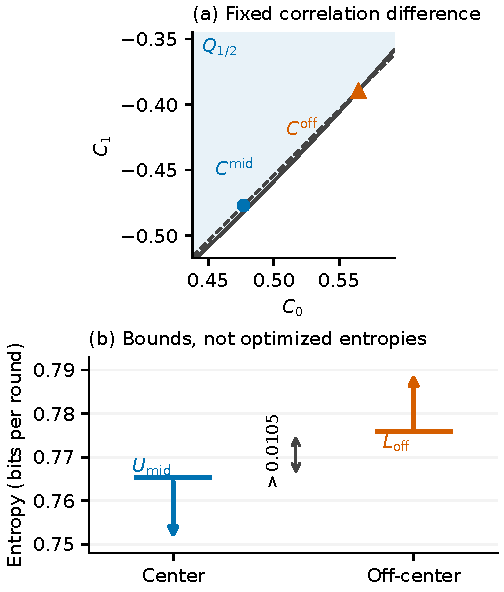
\includegraphics[width=\columnwidth]{figures/bias-gap.pdf}
 \caption{Two correlations with the same difference at $e=1/2$.
 (a) Shading indicates the allowed side of the $Q_{1/2}$ boundary; the dashed
 line has $C_0-C_1=2d$. (b) Horizontal marks give the affine lower bound
 $\Loff$ and feasible upper bound $\Umid$. Arrows show the directions of
 the entropy inequalities; the marks are not optima. AI-assisted
 Python/Matplotlib code generated the plot from analytic equations and
 interval-certificate outputs. Floating-point geometry is for display only.}
 \label{fig:gap}
\end{figure}

\section{A global affine entropy certificate}\label{sec:dual}

All coefficients in the witness below are exact rationals:
\begin{equation}
 t=-\frac{211}{50},\quad b_0=\frac{5907}{100},\quad
 b_1=-\frac{5487}{100},\quad k=\frac{1989}{20}.
 \label{eq:coeff}
\end{equation}
We establish, for every allowed branch,
\begin{equation}
 t+b_0u+b_1v-kw\leq H(u,v).
 \label{eq:affine}
\end{equation}
Averaging this inequality over any feasible ensemble gives
\begin{equation}
 \Hs(C,e)\geq t+b_0C_0+b_1C_1-ke.
 \label{eq:weakdual}
\end{equation}
This is the affine lower-bound principle of the source's Eq.~(32), but
only weak duality is needed here: neither an optimizer nor a strong-duality
theorem enters the proof.

Define $s(a)=h(\cos 2a)$. Because $k>0$, it suffices to use the smallest
allowed branch budget in Eq.~\eqref{eq:angledomain}. Equation~\eqref{eq:affine}
is therefore equivalent to $G(a,b)\geq t$ throughout $[0,\pi/2]^2$, where
\begin{align}
 G(a,b)={}&\tfrac12[s(a)+s(b)]-b_0\cos2a-b_1\cos2b\notag\\
 &+k|a-b|.\label{eq:G}
\end{align}
If $a\geq b$, then $u\leq v$ and
\begin{equation}
 -b_0u-b_1v=-\tfrac{21}{5}u+\tfrac{5487}{100}(v-u)
 \geq-\tfrac{21}{5}>t.
\end{equation}
Since entropy and $k|a-b|$ are nonnegative, this half of the domain is
covered analytically.

If $a\leq b$, the objective separates:
\begin{align}
 G(a,b)&=f_0(a)+f_1(b),\label{eq:sep}\\
 f_0(a)&=\tfrac12s(a)-b_0\cos2a-ka,\notag\\
 f_1(b)&=\tfrac12s(b)-b_1\cos2b+kb.\notag
\end{align}
The following finite computation, with an explicit continuum correction,
covers this entire triangle.

\subsection{Endpoint control and the continuum correction}

Although the derivative of $h(c)$ diverges at $c=\pm1$, the angular entropy
has a bounded derivative. For $0<a<\pi/2$,
\begin{equation}
 s'(a)=\frac{4\sin a\cos a}{\ln2}\ln(\cot a).
\end{equation}
On $0<a\leq\pi/4$, $0\leq\ln(\cot a)\leq-\ln(\sin a)$.
The elementary inequality $-x\ln x\leq1/\exp(1)$ gives
\begin{equation}
 |s'(a)|\leq\frac{4}{\exp(1)\ln2}<3.
\end{equation}
For the last strict bound one can use $\exp(1)>8/3$ and
$\ln2=\int_1^2\dd x/x>1/2$. The symmetry $s(\pi/2-a)=s(a)$
covers the other half, and the one-sided endpoint derivatives tend to zero.
Thus $s$ is globally $3$-Lipschitz, including its endpoints. It follows that
\begin{equation}
 \operatorname{Lip}(f_0)\leq219.09,\qquad
 \operatorname{Lip}(f_1)\leq210.69.
 \label{eq:lipschitz}
\end{equation}
These terminating decimals are exact rational upper bounds.

Take $N=32768$ and $a_j=j\pi/(2N)$, $j=0,\ldots,N$.
Round $a$ and $b$ to the nearest nodes using the same monotone tie rule.
If $a\leq b$, their indices obey $i\leq j$, and each distance is at most
$\pi/(4N)$. Therefore
\begin{align}
 \min_{a\leq b}G(a,b)&\geq M_N-\frac{429.78\pi}{4N},\label{eq:cover}\\
 M_N&=\min_{0\leq i\leq j\leq N}[f_0(a_i)+f_1(a_j)].\notag
\end{align}
There is no unverified interpolation assumption in this estimate.

\subsection{The finite certificate}

Each node value is enclosed by directed interval arithmetic and its lower
endpoint is rounded downward to a multiple of $10^{-25}$. Let the resulting
integers for $f_0$ and $f_1$ be $A_i$ and $B_i$. Then
\begin{equation}
 M_N\geq10^{-25}\min_j\left[B_j+\min_{i\leq j}A_i\right].
 \label{eq:prefix}
\end{equation}
The inner minimum is maintained as a running prefix minimum. This evaluates
the bound for all ordered node pairs in linear time without omitting any pair.
The full traversal gives
\begin{equation}
 M_N\geq-\frac{42067321733044440200715843}{10^{25}}.
 \label{eq:gridnumber}
\end{equation}
Using $\pi<22/7$, the continuum correction is bounded by
\begin{equation}
 E_N=\frac{236379}{22937600}.
\end{equation}
Combining this with Eqs.~\eqref{eq:cover} and~\eqref{eq:gridnumber} yields
\begin{equation}
 \begin{aligned}
 \min_{a\leq b}G(a,b)&\geq
 -\frac{295192623591272018905010901}{7\cdot10^{25}}\\
 &>-4.22.
 \end{aligned}
 \label{eq:globalnumber}
\end{equation}
Together with the analytic reverse triangle, this proves
Eq.~\eqref{eq:affine} over the full branch domain. The same discrete integer
bound was obtained with 40-digit \texttt{mpmath.iv} intervals and a separate
48-digit Decimal implementation. A third implementation using 128-bit
fixed-point integer intervals checks continuous cells directly and avoids
the Lipschitz correction; see Appendix~\ref{app:arithmetic}.

Evaluating Eq.~\eqref{eq:weakdual} at $\Coff$ gives
\begin{align}
 \Loff={}&-4.22+59.07\sin(3/5)+54.87\sin(2/5)\notag\\
 &-99.45/2>0.7758,
 \label{eq:L}
\end{align}
which proves Eq.~\eqref{eq:offbound}.

\section{An exactly feasible center ensemble}\label{sec:primal}

Choose
\begin{equation}
 w=\frac{66}{125},\qquad q=\frac{d}{\sin w},\qquad
 w_0=\frac{1/2-qw}{1-q}.
 \label{eq:ensemblepars}
\end{equation}
Consider the three branches in Table~\ref{tab:ensemble}.
Their weights are legitimate because interval evaluation gives
\begin{equation}
 0.94685<q<0.94686,\qquad 0.00116<w_0<0.00118.
 \label{eq:feasible}
\end{equation}
The anticorrelated branch has minimum budget exactly $w$. The other two
branches are deterministic and lie in $Q_{w_0}$ for any nonnegative $w_0$.
Their budget labels need not be saturated by their actual energy uncertainties.

\begin{table}[b]
 \caption{A feasible ensemble for $(\Cmid,e)$. All weights and budget
 parameters have the exact definitions in Eq.~\eqref{eq:ensemblepars}.}
 \label{tab:ensemble}
 \begin{ruledtabular}
 \begin{tabular}{ccc}
 Probability & Correlations & Budget\\
 \hline
 $q$ & $(\sin w,-\sin w)$ & $w$\\
 $(1-q)/2$ & $(1,1)$ & $w_0$\\
 $(1-q)/2$ & $(-1,-1)$ & $w_0$
 \end{tabular}
 \end{ruledtabular}
\end{table}

The moment constraints hold as algebraic identities:
\begin{equation}
 q\sin w=d,\qquad qw+(1-q)w_0=1/2.
\end{equation}
The two deterministic contributions cancel in the correlation mean and
contribute zero entropy. Hence
\begin{equation}
 \Hs(\Cmid,1/2)\leq\Umid:=q\,h(\sin w)<0.7653.
 \label{eq:U}
\end{equation}
This proves Eq.~\eqref{eq:midbound}. Feasibility is exact, not equality
within a linear-programming tolerance. Neither the three-branch support
nor the chosen $w$ is asserted to be optimal.

For clarity, outward-rounded interval evaluations of the two witness values
and their difference give
\begin{align}
 0.77581534592039102759&<\Loff\notag\\
 &<0.77581534592039102760,\notag\\
 0.76529069411815580216&<\Umid\notag\\
 &<0.76529069411815580217,\label{eq:scalarintervals}\\
 0.01052465180223522542&<\Loff-\Umid\notag\\
 &<0.01052465180223522543.\notag
\end{align}
These narrow intervals describe $\Loff$ and $\Umid$, not the two optimized
entropies. The asserted separation in Eq.~\eqref{eq:gap} uses only the
coarser strict bounds.

\section{Physical interpretation and scope}\label{sec:scope}

For quantum-admissible data, replacing the off-center correlations by their
center can lose more than $0.0105$ bits per round in Eq.~\eqref{eq:roof}.
The inequality in Eq.~\eqref{eq:centerlemma} remains valid: center bounds
may still be propagated along lines of fixed correlation difference as
conservative bounds, including the use described in Appendix~E(v) of
Ref.~\cite{JonesSpeed2026}. The counterexample concerns the conjectured
equality, not that lower-bound procedure.

It is essential to distinguish the average branch constraint from a bound
on the energy uncertainty of the total prepared state. For a fixed
Hamiltonian $K$ and $\bar\rho=\sum_\lambda p_\lambda\rho_\lambda$,
\begin{align}
 \operatorname{Var}_{\bar\rho}(K)
 ={}&\sum_\lambda p_\lambda\operatorname{Var}_{\rho_\lambda}(K)\notag\\
 &+\operatorname{Var}_{p}\!\left(\operatorname{tr}\rho_\lambda K\right).
\end{align}
Consequently $\Delta K_{\bar\rho}\geq\sum_\lambda p_\lambda\Delta K_{\rho_\lambda}$.
A total-state uncertainty bound therefore implies an average branch bound;
the reverse implication is not automatic. Our center ensemble establishes
an upper bound for Eq.~\eqref{eq:roof}, not an optimal physical attack under
the stronger total-state constraint.

Nor can one directly identify the average speed budget with the earlier
average-energy constraints of Ref.~\cite{VanHimbeeck2019}. That work retains
input-dependent energy expectation bounds and permits full-statistics or
linear-statistic entropy optimization; see its version-1 Eqs.~(26)--(29)
and Remark~9. The constraints are not the scalar average of $w$ used here.
Even if an individual overlap can be matched by an energy parameter
$\omega=\sin^2(w/2)$, this nonlinear change does not preserve ensemble averages.
Likewise, the comparison to energy constraints in Appendix~E of
Ref.~\cite{JonesSpatial2026}, Eqs.~(55)--(58), explicitly treats a regime
without a maximum-average assumption. That peak-constraint correspondence
does not establish equality for the average speed problem.

The result is a single strict counterexample, with no claim of a phase
diagram, exact optimized entropy, new duality method, or exhaustive priority
over subsequent literature. It assumes classical side information and does
not provide a quantum-side-information or finite-sample security proof.
There is no spatial boundary, thermodynamic limit, perturbative order, or
uncontrolled infinite-dimensional tail in the certificate. Extending the
comparison to the true total-state constraint is a separate question.

\section{Computation and reproducibility}\label{sec:compute}

The reproducibility files contain the fixed rational coefficients, the
analytic ensemble definitions, and standalone Decimal and integer checkers.
Both recompute the global witness and scalar bounds without external
numerical packages or cached function values. The verified
environment is Python~3.9.6; the Decimal backend is version~1.70 with
libmpdec~2.5.0. The integer checker uses only Python integer and rational
arithmetic. Computational correctness relies on those arithmetic
implementations and the explicit error arguments, and has not been
formalized in a proof assistant.

AI assistance was substantive: OpenAI Codex was used for literature
comparison, counterexample search, derivations, certificate code, numerical
checks, and interpretation. The writing environment
identifies its model as GPT-6; exact model revisions across the earlier
research sessions have not been independently established. Separately
implemented arithmetic checks provide the computational cross-checks
described above. They do not constitute external peer review. Human
scientific review and approval of this local draft remain pending.

\begin{acknowledgments}
OpenAI Codex, identified as GPT-6 in the writing environment, also assisted
with drafting and revising the manuscript, bibliography preparation, and
figure code. Its research contributions and verification limits are
described in Sec.~\ref{sec:compute}.
\end{acknowledgments}

\section*{Data availability}
All data needed to reproduce the stated bounds are specified in the paper
and the accompanying local reproducibility files. These include two
standalone checkers, certificate outputs, a figure script, and instructions.
No external experimental dataset is used. A public archive location has not
yet been assigned.

\appendix
\section{Arithmetic and an independent continuous-cell bound}\label{app:arithmetic}

\subsection{Directed Decimal node evaluation}

The Decimal checker uses 48-digit outward rounding for addition,
multiplication, and division. It encloses $\pi$ through
\begin{equation}
 \pi=16\arctan(1/5)-4\arctan(1/239),
\end{equation}
using 40 terms of each rational alternating series and the next-term
remainder. Cosine is evaluated through degree~58 and sine through
degree~59, with absolute remainder bounds
$(22/7)^{60}/60!$ and $(22/7)^{61}/61!$, respectively. The logarithm of
each interval endpoint is evaluated by Decimal's correctly rounded
nearest logarithm~\cite{PythonDecimal}, then widened to its neighboring representable numbers.
Monotonicity encloses the logarithm throughout the input interval.
Probabilities are reconstructed as $(1\pm\cos2a)/2$; at the two exact
endpoints the entropy is set to zero. This gives all $A_i,B_i$ of
Eq.~\eqref{eq:prefix} by exact conversion of decimal endpoints to rationals
followed by downward integer rounding.

\subsection{Direct interval-cell coverage}

An independently implemented check avoids the nearest-node and Lipschitz
arguments altogether. Partition $[0,\pi/2]$ into $n=65536$ cells
$I_j=[\alpha_j,\alpha_{j+1}]$, with $\alpha_j=j\pi/(2n)$.
The entropy $s$ increases up to $\pi/4$ and decreases afterwards. Set
\[
 m_j=\min\{s(\alpha_j),s(\alpha_{j+1})\}.
\]
This smaller endpoint value bounds $s$ below throughout the cell, including
a cell containing the maximum. Cosine decreases over the angular range.
It follows
that, for every $\theta\in I_j$,
\begin{align}
 f_0(\theta)&\geq\tfrac12m_j-b_0\cos2\alpha_j-k\alpha_{j+1}
 =:\mathcal A_j,\notag\\
 f_1(\theta)&\geq\tfrac12m_j-b_1\cos2\alpha_{j+1}+k\alpha_j
 =:\mathcal B_j.
 \label{eq:cells}
\end{align}
Choosing cell indices monotonically, with $\pi/2$ assigned to the last
cell, ensures $i\leq j$ whenever $a\leq b$. Therefore
\begin{equation}
 \min_{a\leq b}G(a,b)\geq
 \min_j\left[\mathcal B_j+\min_{i\leq j}\mathcal A_i\right].
 \label{eq:cellprefix}
\end{equation}
The same-cell rectangle may include points outside the triangle, but this
only lowers the bound. The prefix algorithm again covers every ordered
pair, using $O(n)$ work and constant auxiliary storage.

This implementation represents interval endpoints as integers divided by
$S=2^{128}$, rounding outward after every operation. It encloses $\pi$ by
$4[\arctan(1/2)+\arctan(1/3)]$ with 80 rational alternating terms in each
arctangent. Cosine uses the Taylor polynomial through degree~48 and remainder
$(22/7)^{50}/50!$. For logarithms, powers of two reduce a positive argument
to $y\geq1$; the code verifies $0\leq z=(y-1)/(y+1)\leq1/2$ and uses
\begin{equation}
 \ln y=2\sum_{j=0}^{55}\frac{z^{2j+1}}{2j+1}+R,
 \qquad 0\leq R\leq\frac{8}{3\cdot113\cdot2^{113}}.
\end{equation}
The same series encloses $\ln2$ and reconstructs the original logarithm.
This backend calls no floating-point trigonometric or logarithmic function.

The complete traversal gives $\min_{a\leq b}G(a,b)\geq R_{\rm cell}$, where
the conservative bound is the exact rational number
\begin{equation}
 R_{\rm cell}=
 -\frac{1433099017456186434282593190730506873727}
 {2^{128}}.
 \label{eq:integercell}
\end{equation}
It is greater than $-4.211500$ and hence greater than $t=-4.22$.
This independently certifies the unchanged witness. The same integer
arithmetic yields Eq.~\eqref{eq:scalarintervals}. No part of the conclusion
depends on agreement of unbounded-precision decimal approximations alone.

\bibliography{references}
\end{document}
